\documentclass[wide,a4paper,titlepage,12pt]{mwart}
\usepackage{polski,graphicx,pdflscape}
\usepackage[utf8]{inputenc}
\usepackage{listings}


\title{Badanie podstawowych parametrów sygnałów}
\author{Tymon Tobolski (181037)\\\small Jacek Wieczorek (181043)}

% Title page layout (fold)
\makeatletter
\renewcommand{\maketitle}{
\begin{titlepage}
  \begin{center}
    \vspace*{3cm}
    \LARGE \@title \par
    \vspace{2cm}
    \textit{\small Autor:}\par
    \normalsize \@author\par \normalsize
    \vspace{3cm}
    \textit{\small Prowadzący:}\par
    Dr inż. Paweł Biernacki \par
    \vspace{2cm}
    Wydział Elektroniki\\ II rok\\ WT/TN 13:15--15:00 \par
    \vspace{5cm}
    \small \@date
  \end{center}
\end{titlepage}
}
\makeatother
% Title page layout (end)

\begin{document}
  \maketitle
  \section{Cel ćwiczenia} % (fold)
  \label{sec:Cel}
    Celem ćwiczenia jest sprawdzenie podstawowych parametrów sygnałów deterministycznych. 
    
  \section{Parametry sygnałów}
    Na początku wygenerowaliśmy dwa sygnały o nastepujących parametrach:
    \begin{itemize}
      \item prostokątny ($A=10, f=2, fpr=100, faza=0, T=2, \omega=0.5$) 
      \item trójkątny ($A=10, f=2, fpr=100, faza=0, T=2, \omega=0.5$)
    \end{itemize}
    
    \begin{figure}[htbp]
      \begin{center}
        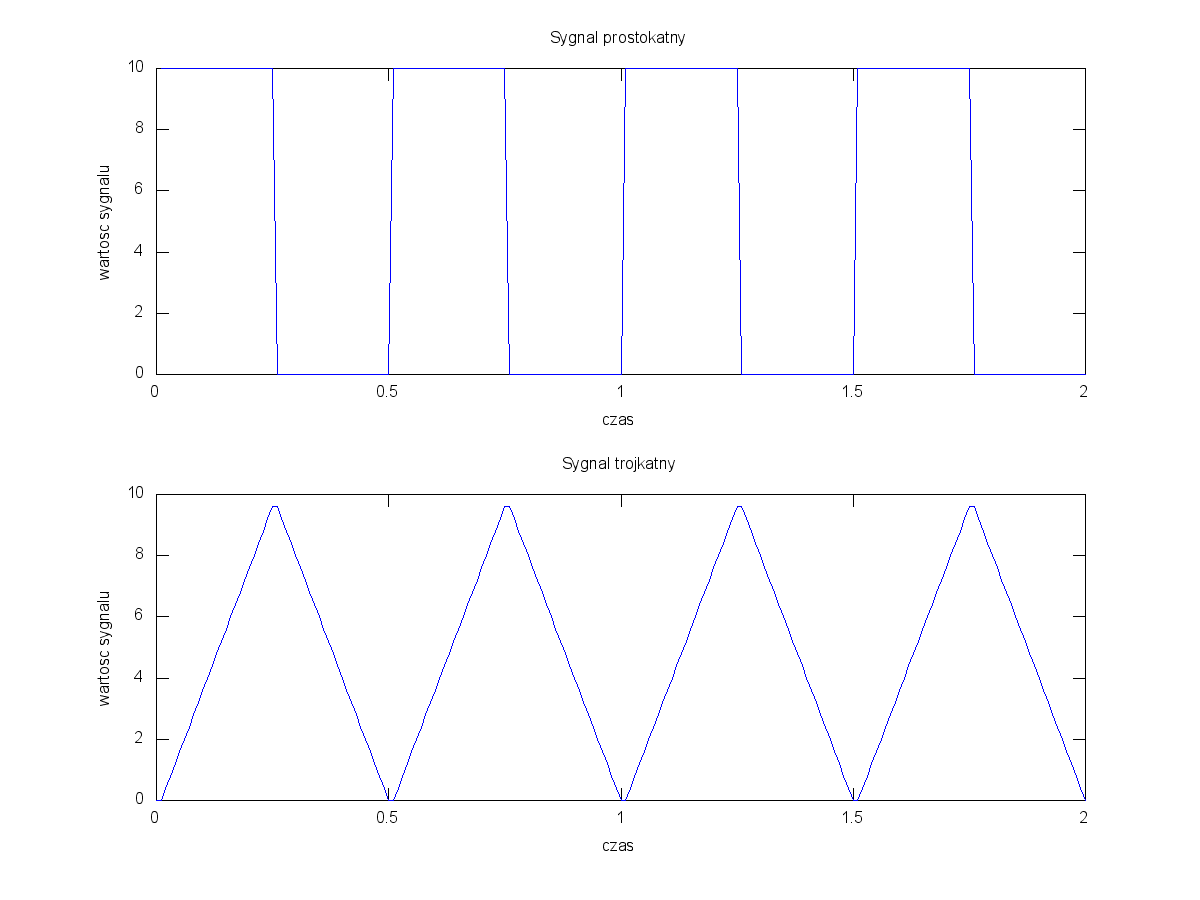
\includegraphics[scale=.4]{out/Figure1.png}
        \caption{\label{wykres1}Badane sygnały.}
      \end{center}
    \end{figure}
    
  \section{Algorytm przetwarzający}
    Wykorzystuje dostarczone funkcje:
    \newline
    \begin{itemize}
      \item generujące sygnał (\textbf{prostokat}, \textbf{trojkat})
      \item obliczające wartość średnią (\textbf{wart\_srednia}, \textbf{chwil\_wart\_sred}, \textbf{biez\_wart\_sred})
      \item obliczające wariancje (\textbf{wariancja}, \textbf{chwil\_wariancja}, \textbf{biez\_wariancja})
    \end{itemize}
  
  \lstset{ %
    language=Octave,                % choose the language of the code
    basicstyle=\scriptsize,       % the size of the fonts that are used for the code
    numbers=left,                   % where to put the line-numbers
    numberstyle=\scriptsize,      % the size of the fonts that are used for the line-numbers
    stepnumber=10,                   % the step between two line-numbers. If it's 1 each line 
                                    % will be numbered
    numbersep=9pt,                  % how far the line-numbers are from the code
    % backgroundcolor=\color{white},  % choose the background color. You must add \usepackage{color}
    showspaces=false,               % show spaces adding particular underscores
    showstringspaces=false,         % underline spaces within strings
    showtabs=false,                 % show tabs within strings adding particular underscores
    % frame=single,                 % adds a frame around the code
    % tabsize=2,                  % sets default tabsize to 2 spaces
    % captionpos=b,                   % sets the caption-position to bottom
    breaklines=true,                % sets automatic line breaking
    % breakatwhitespace=false,        % sets if automatic breaks should only happen at whitespace
    % title=\lstname,                 % show the filename of files included with \lstinputlisting;
                                    % also try caption instead of title
    % escapeinside={\%*}{*)},         % if you want to add a comment within your code
    % morekeywords={*,...}            % if you want to add more keywords to the set
    }
    \lstinputlisting{lab1.m}
    
  % section Wstęp (end)
  
  \section{Parametry opisujące sygnał}
    \subsection{Wartość średnia}
      \begin{displaymath}
        m = \frac{1}{Len} \sum^{Skip+Len-1}_{i=Skip} x(i)
      \end{displaymath}
      Przedział wartości fazy: $faza \in \left \{0,10,20,30,40,50,60,70,80,90,100\right \}$
      \newline
      Przedział wartości wypełnienia: $\omega \in \left \{0, 0.1, 0.2, 0.3, 0.4, 0.5, 0.6, 0.7, 0.8, 0.9, 1.0\right \}$
      \newline
      
      \begin{table}[h]
        \begin{center}
          \begin{tabular}{|c|c|c|c|c|c|}
            \hline
              $faza$ &
              \multicolumn{2}{|c|}{Wartość średnia} &
              $\omega$ &
              \multicolumn{2}{|c|}{Wartość średnia} \\
               & prostokątny & trójkątny & & prostokątny & trójkątny \\
            \hline
              0 & 5 & 4.8   & 0.0 & 0 & 4.8 \\
              10 & 5 & 4.8   & 0.1 & 1 & 4.8 \\
              20 & 5 & 4.8   & 0.2 & 2 & 4.8 \\
              30 & 5 & 4.8   & 0.3 & 3 & 4.8 \\
              40 & 5 & 4.8   & 0.4 & 4 & 4.8 \\
              50 & 5 & 4.8   & 0.5 & 5 & 4.8 \\
              60 & 5 & 4.8   & 0.6 & 6 & 4.8 \\
              70 & 5 & 4.8   & 0.7 & 7 & 4.8 \\
              80 & 5 & 4.8   & 0.8 & 8 & 4.8 \\
              90 & 5 & 4.8   & 0.9 & 9 & 4.8 \\
              100 & 5 & 4.8   & 1.0 & 10 & 4.8 \\
            \hline
          \end{tabular}
        
          \caption{Wartość średnia sygnałów w zależności od $fazy$ i $\omega$.}
        \end{center}
      \end{table}
      
      Wykresy znajdują się na stronie \pageref{wykres2}
    
    \subsection{Chwilowa wartość średnia}
      \begin{displaymath}
        m(j) = \frac{1}{k} \sum^{j}_{i=j-k+1} x(i)
      \end{displaymath}
      Przedział: $k \in (1 ; N)$
      \newline
      Wykresy znajdują się na stronie \pageref{wykres3} oraz \pageref{wykres4}
    
    \subsection{Bieżąca wartość średnia}
      \begin{displaymath}
        m(j) = \alpha m(j-1) + (1-\alpha) x(j)
      \end{displaymath}
      Przedział: $\alpha \in \left \{0.1, 0.3, 0.5, 0.7, 0.9, 0.92, 0.95, 0.99, 0.999, 1.0\right \}$
      \newline
      Wykresy znajdują się na stronie \pageref{wykres5} oraz \pageref{wykres6}
      
    \subsection{Wariancja}
      \begin{displaymath}
        v = \frac{1}{Len} \sum^{Skip+Len-1}_{i=Skip} [x(i)-m]^2
      \end{displaymath}
      Przedział wartości fazy: $faza \in \left \{0,10,20,30,40,50,60,70,80,90,100\right \}$
      \newline
      Przedział wartości wypełnienia: $\omega \in \left \{0, 0.1, 0.2, 0.3, 0.4, 0.5, 0.6, 0.7, 0.8, 0.9, 1.0\right \}$
      \newline
      
      \begin{table}[h]
        \begin{center}
          \begin{tabular}{|c|c|c|c|c|c|}
            \hline
              $faza$ &
              \multicolumn{2}{|c|}{Wariancja} &
              $\omega$ &
              \multicolumn{2}{|c|}{Wariancja} \\
               & prostokątny & trójkątny & & prostokątny & trójkątny \\
            \hline
              0   & 25 & 8.32   & 0.0 & 0  & 8.32 \\
              10  & 25 & 8.32   & 0.1 & 9  & 8.32 \\
              20  & 25 & 8.32   & 0.2 & 16 & 8.32 \\
              30  & 25 & 8.32   & 0.3 & 21 & 8.32 \\
              40  & 25 & 8.32   & 0.4 & 24 & 8.32 \\
              50  & 25 & 8.32   & 0.5 & 25 & 8.32 \\
              60  & 25 & 8.32   & 0.6 & 24 & 8.32 \\
              70  & 25 & 8.32   & 0.7 & 21 & 8.32 \\
              80  & 25 & 8.32   & 0.8 & 16 & 8.32 \\
              90  & 25 & 8.32   & 0.9 & 9  & 8.32 \\
              100 & 25 & 8.32   & 1.0 & 0  & 8.32 \\
            \hline
          \end{tabular}
        
          \caption{Wariancja sygnałów w zależności od $fazy$ i $\omega$.}
        \end{center}
      \end{table}
      
      Wykresy znajdują się na stronie \pageref{wykres7}
      
    \subsection{Chwilowa wariancja}
      \begin{displaymath}
        v(j) = \frac{1}{k} \sum^{j}_{i=j-k+1} [x(i)-m(j)]^2
      \end{displaymath}
      Przedział: $k \in (1 ; N)$
      \newline
      Wykresy znajdują się na stronie \pageref{wykres8} oraz \pageref{wykres9}
      
    \subsection{Bieżąca wariancja}
      \begin{displaymath}
        m(j) = \alpha v(j-1) + (1-\alpha) [x(j) - m(j)]^2
      \end{displaymath}
      Przedział: $\alpha \in \left \{0.1, 0.3, 0.5, 0.7, 0.9, 0.92, 0.95, 0.99, 0.999, 1.0\right \}$
      \newline
      Wykresy znajdują się na stronie \pageref{wykres10} oraz \pageref{wykres11}
      
      
      \begin{landscape}
        \begin{figure}[htbp]
          \begin{center}
            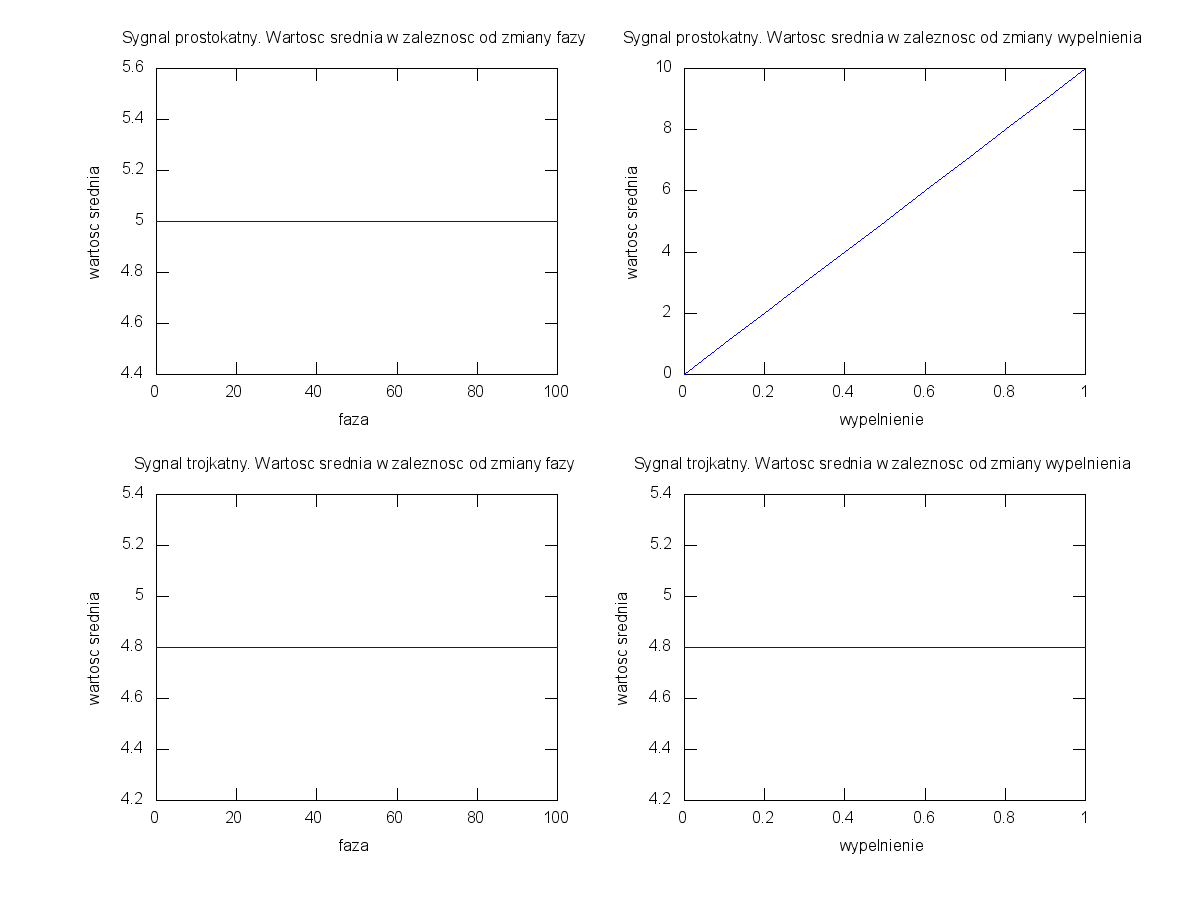
\includegraphics[scale=.5]{out/Figure2.png}
            \caption{\label{wykres2}Wartość średnia sygnałów w zależności od zmiany wypełnienia i fazy.}
          \end{center}
        \end{figure}
      \end{landscape}

      \begin{landscape}
        \begin{figure}[htbp]
          \begin{center}
            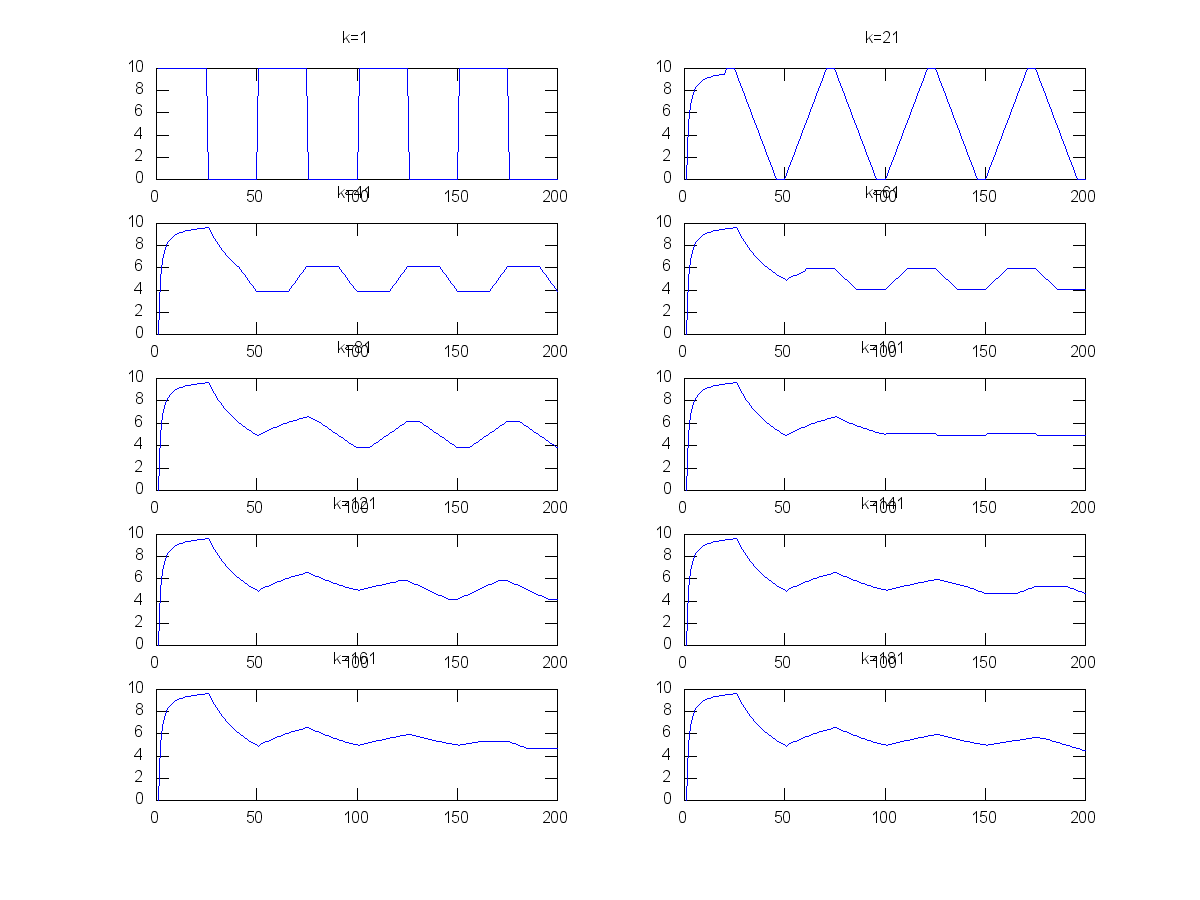
\includegraphics[scale=.5]{out/Figure3.png}
            \caption{\label{wykres3}Sygnał prostokątny, chwilowa wartość średnia. $N=200$}
          \end{center}
        \end{figure}
      \end{landscape}

      \begin{landscape}
        \begin{figure}[htbp]
          \begin{center}
            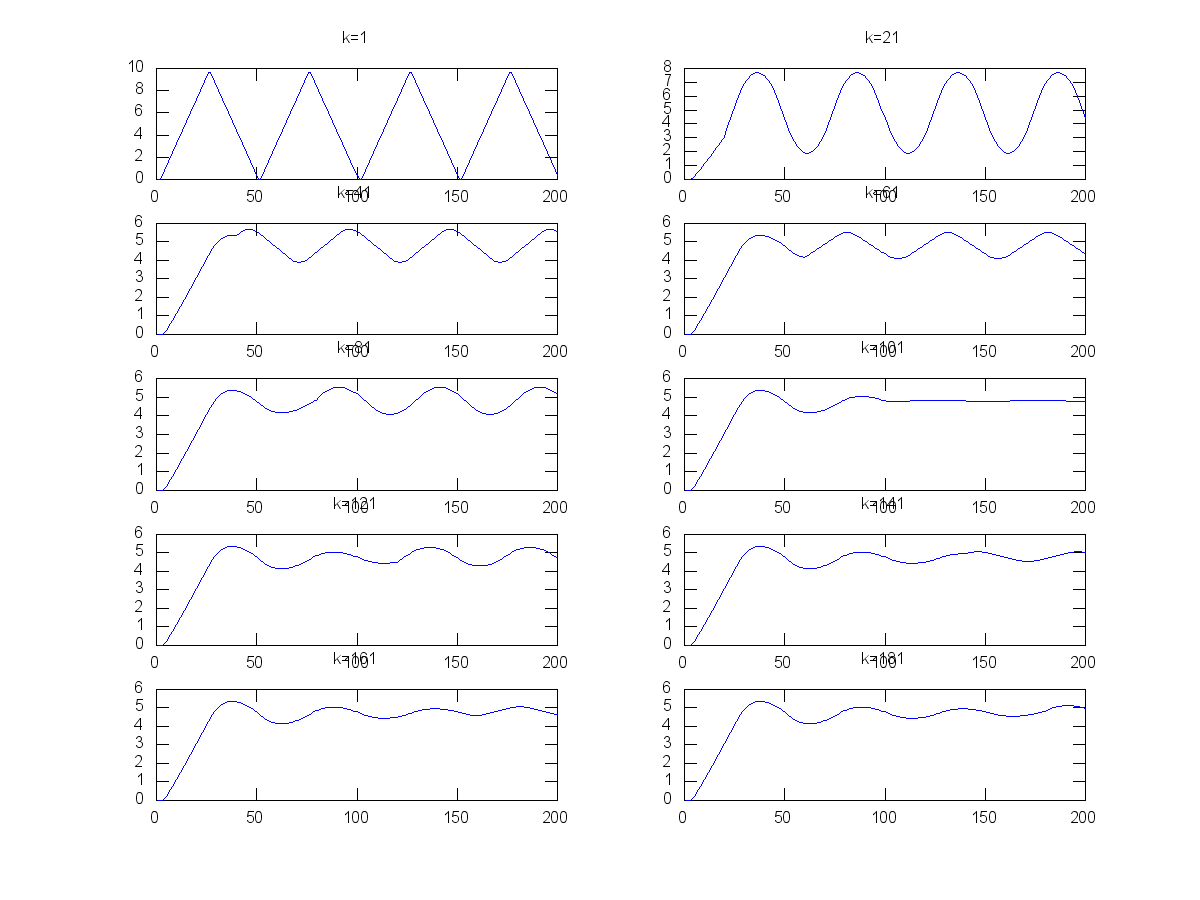
\includegraphics[scale=.5]{out/Figure4.png}
            \caption{\label{wykres4}Sygnał trójkątny, chwilowa wartość średnia. $N=200$}
          \end{center}
        \end{figure}
      \end{landscape}

      \begin{landscape}
        \begin{figure}[htbp]
          \begin{center}
            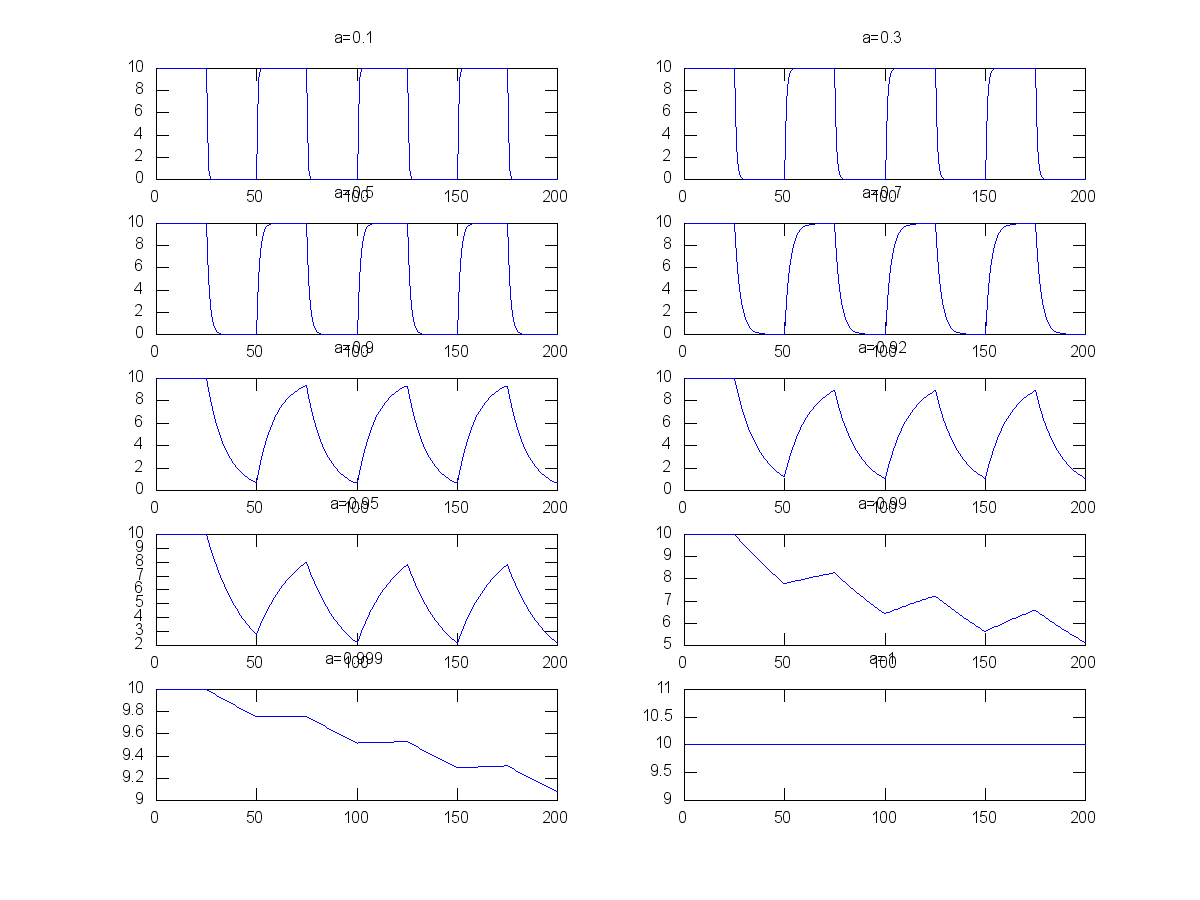
\includegraphics[scale=.5]{out/Figure5.png}
            \caption{\label{wykres5}Sygnał prostokątny, bieżąca wartość średnia. $N=200$}
          \end{center}
        \end{figure}
      \end{landscape}

      \begin{landscape}
        \begin{figure}[htbp]
          \begin{center}
            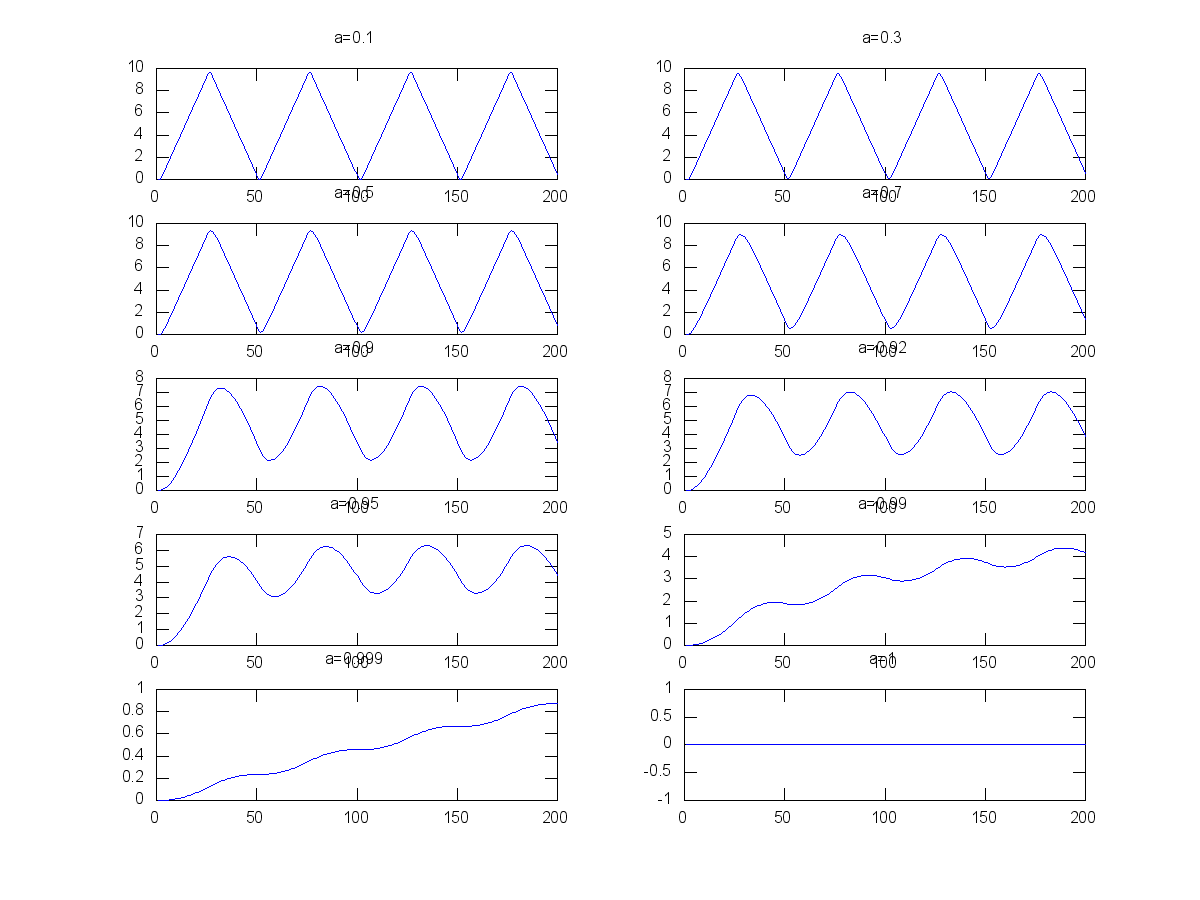
\includegraphics[scale=.5]{out/Figure6.png}
            \caption{\label{wykres6}Sygnał trójkątny, bieżąca wartość średnia. $N=200$}
          \end{center}
        \end{figure}
      \end{landscape}

      \begin{landscape}
        \begin{figure}[htbp]
          \begin{center}
            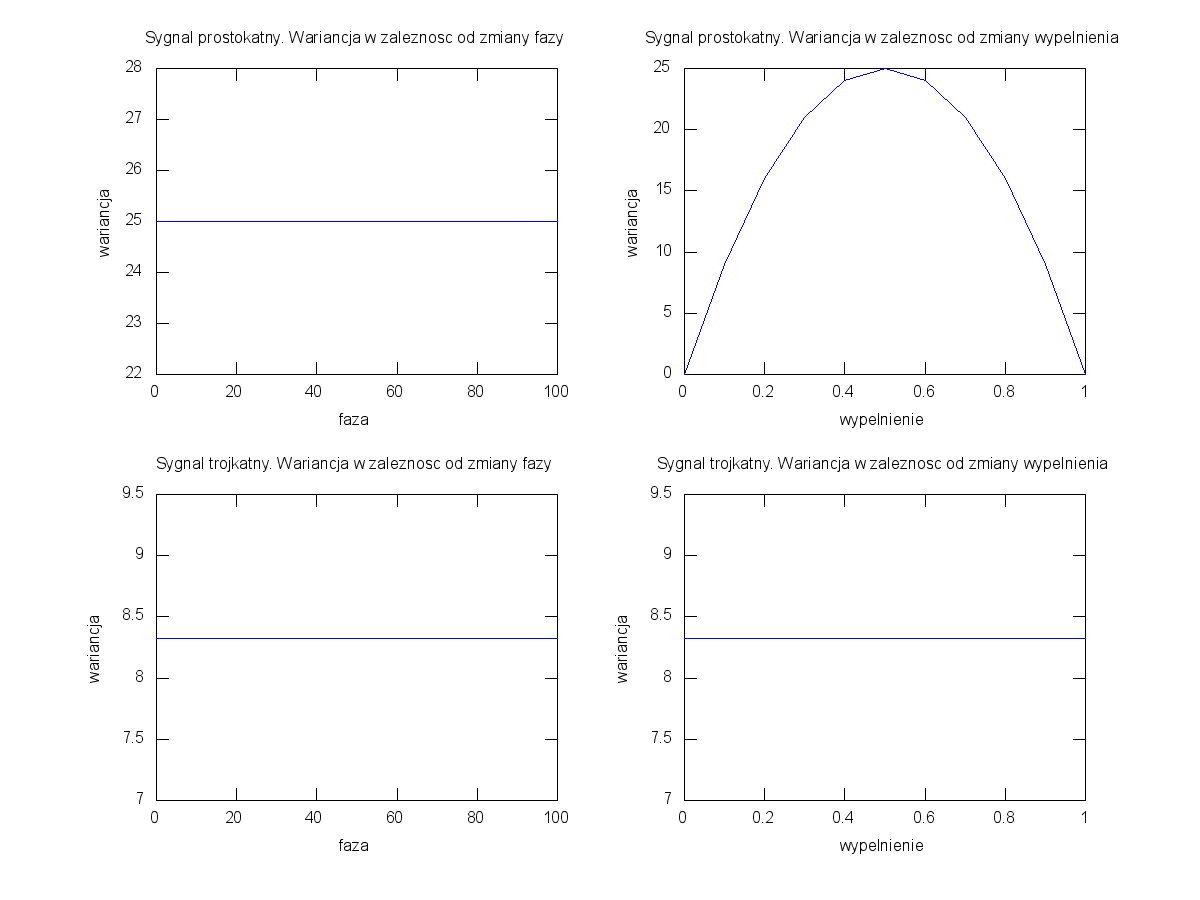
\includegraphics[scale=.5]{out/Figure7.png}
            \caption{\label{wykres7}Wariancja sygnałów w zależności od zmiany wypełnienia i fazy.}
          \end{center}
        \end{figure}
      \end{landscape}


      \begin{landscape}
        \begin{figure}[htbp]
          \begin{center}
            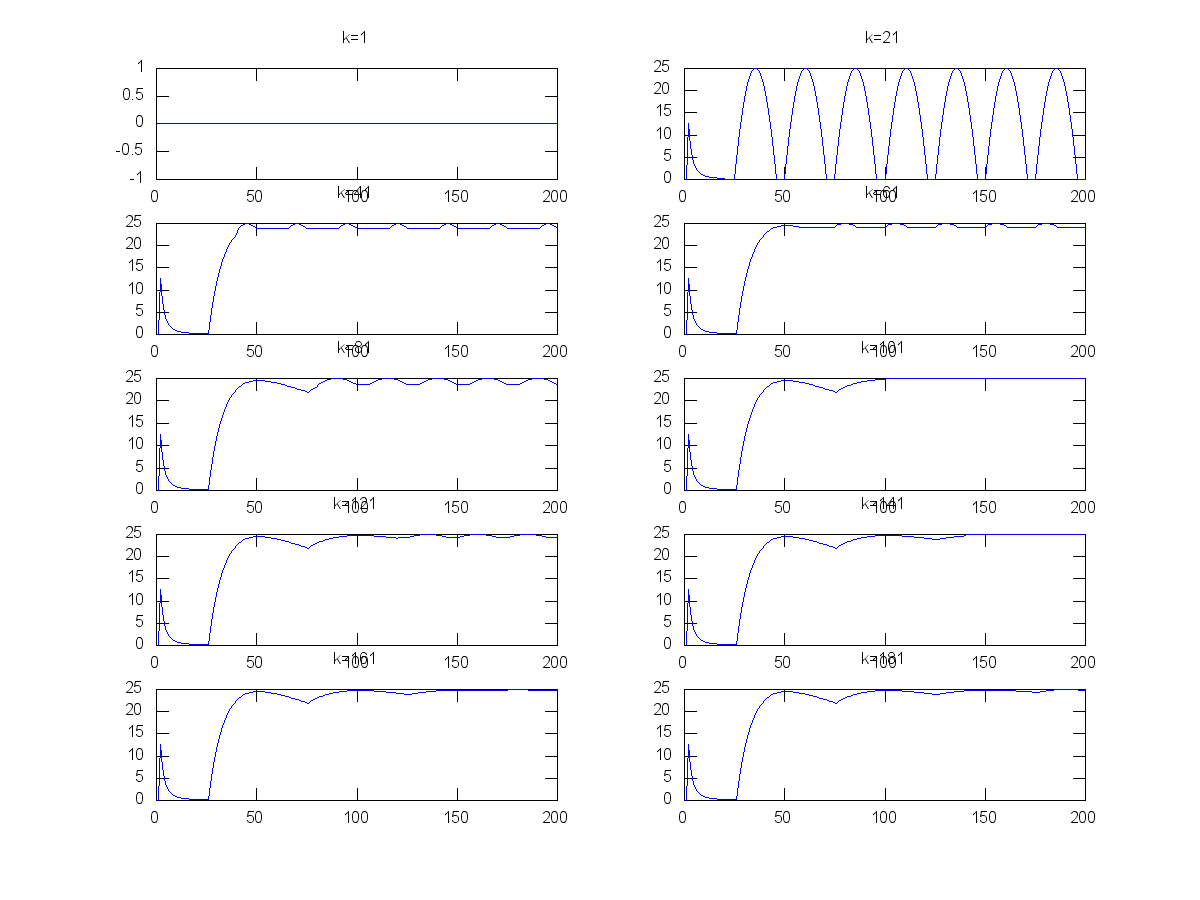
\includegraphics[scale=.5]{out/Figure8.png}
            \caption{\label{wykres8}Sygnał prostokątny, chwilowa wariancja. $N=200$}
          \end{center}
        \end{figure}
      \end{landscape}

      \begin{landscape}
        \begin{figure}[htbp]
          \begin{center}
            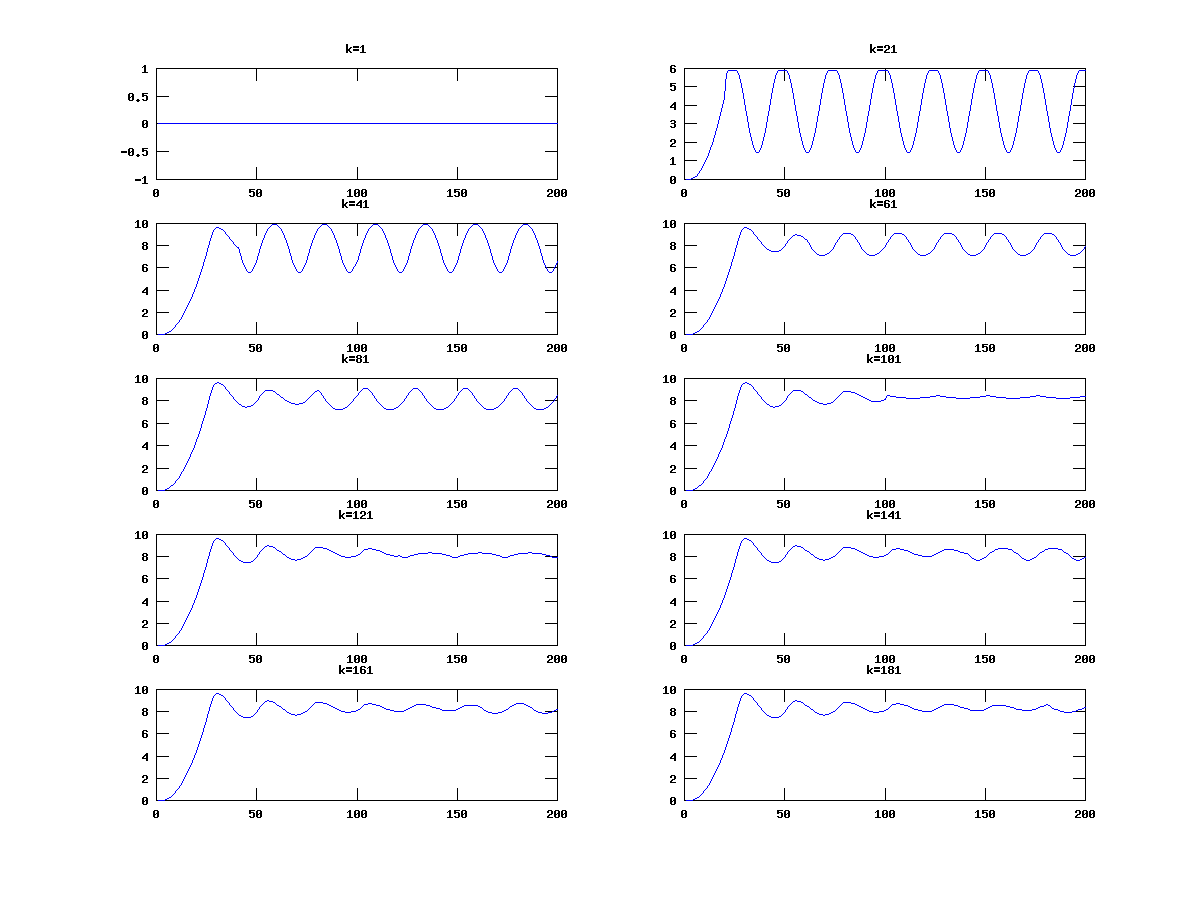
\includegraphics[scale=.5]{out/Figure9.png}
            \caption{\label{wykres9}Sygnał trójkątny, chwilowa wariancja. $N=200$}
          \end{center}
        \end{figure}
      \end{landscape}

      \begin{landscape}
        \begin{figure}[htbp]
          \begin{center}
            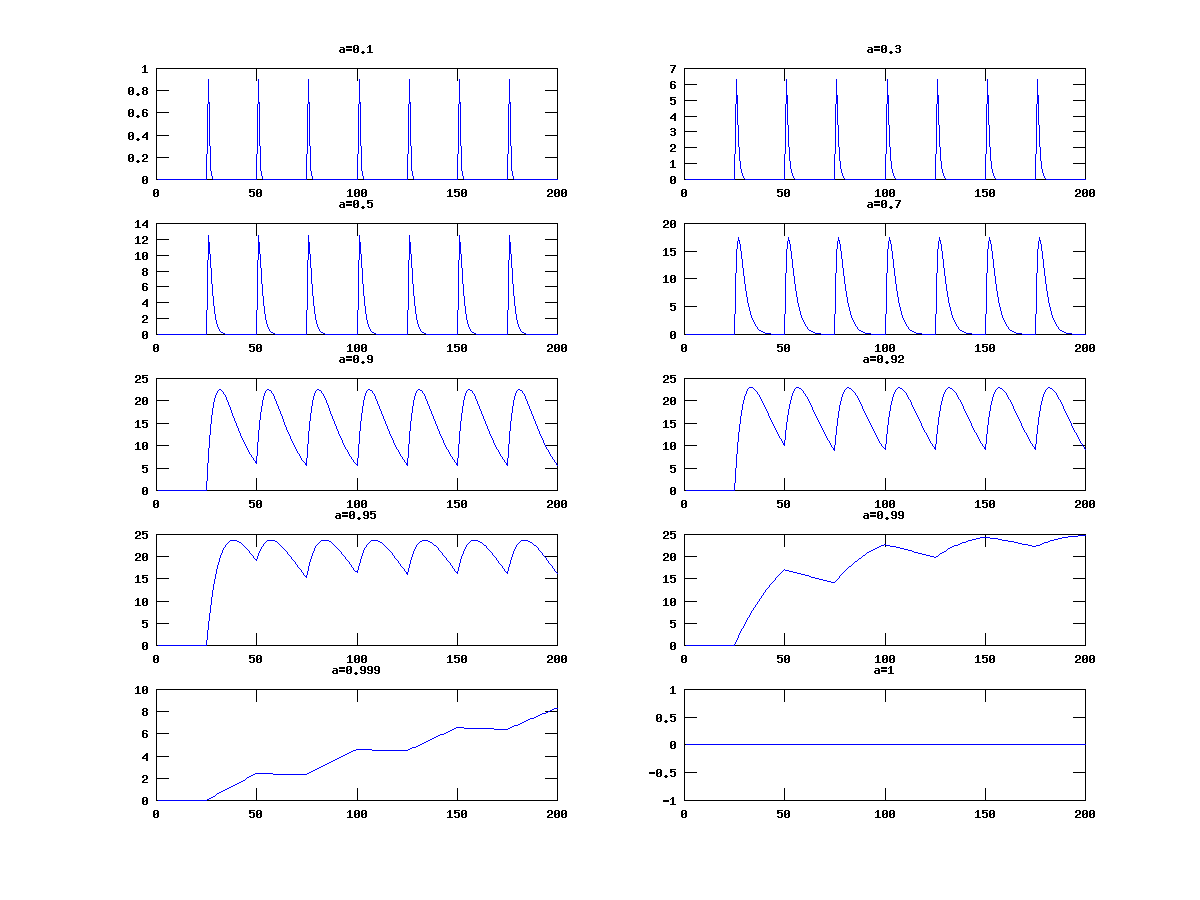
\includegraphics[scale=.5]{out/Figure10.png}
            \caption{\label{wykres10}Sygnał prostokątny, bieżąca wariancja. $N=200$}
          \end{center}
        \end{figure}
      \end{landscape}

      \begin{landscape}
        \begin{figure}[htbp]
          \begin{center}
            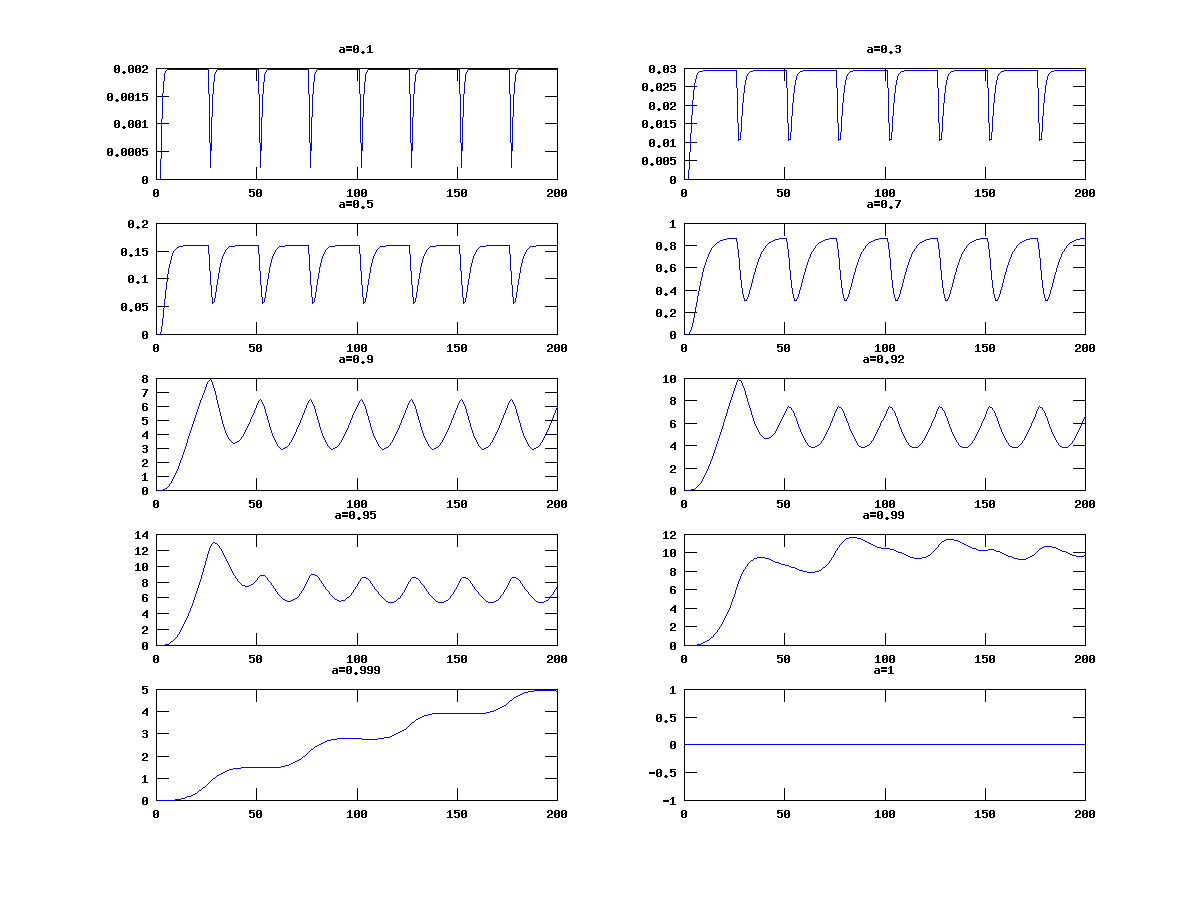
\includegraphics[scale=.5]{out/Figure11.png}
            \caption{\label{wykres11}Sygnał trójkątny, bieżąca wariancja. $N=200$}
          \end{center}
        \end{figure}
      \end{landscape}
      
        
  \section{Wnioski}
  \label{sec:Wnioski}
    \subsection{Wartość średnia}
    Jako pierwszą obliczaliśmy wartość średnią sygnałów w zależności od zmiany fazy i wypełnienia. Zarówno w sygnale prostokątnym, jak i trójkątnym, zmiana fazy nie powodowała zmiany wartości średniej. Natomiast zmiana wypełnienia (zwiększąło się) powodowała liniowy wzrost wartości średniej sygnału prostokątnego. Wartośc średnia sygnału trójkątnego, mimo zmiany wypełnienia nie zmieniła się. 

    \subsection{Chwilowa wartość średnia}
    Wraz ze wzrostem ilości próbek $k$ sygnałów prostokątnego i trójkątnego, wykres chwilowej średniej sygnału, coraz bardziej dążył do funkcji stałej, o amplitudzie równej wartości średniej sygnału.

    \subsection{Bieżąca wartość średnia}
    Wraz ze wzrostem stałej adpatacji $a \rightarrow 1$, wykres wartości  średniej  bieżącej sygnału dąży do funkcji stałej.

    \subsection{Wariancja}
    Wariancja sygnałów w zależności od zmiany fazy i wypełnienia. Zarówno w sygnale prostokątnym, jak i trójkątnym, zmiana fazy nie powodowała zmiany wartości . Natomiast zmiana wypełnienia (zwiększało się) powoduje, że wariancja sygnału prostokątnego jest funkcją kwadratową. Wartośc wariancji sygnału trójkątnego, mimo zmiany wypełnienia nie zmieniła się. 

    \subsection{Chwilowa wariancja}
    Wraz ze wzrostem ilości próbek k sygnałów prostokątnego i trójkątnego, wykres chwilowej wariancji sygnału, coraz bardziej dążył do swojej wariancji.

    \subsection{Bieżąca wariancja}
    Wraz ze wzrostem stałej adpatacji $a \rightarrow 1$, wykres wartości bieżącej wariancji sygnału dąży do funkcji stałej.


  % section Wnioski (end)

% Wykresy (fold)
  %   \begin{landscape}
  %   \begin{figure}[htbp]
  %     \begin{center}
  %       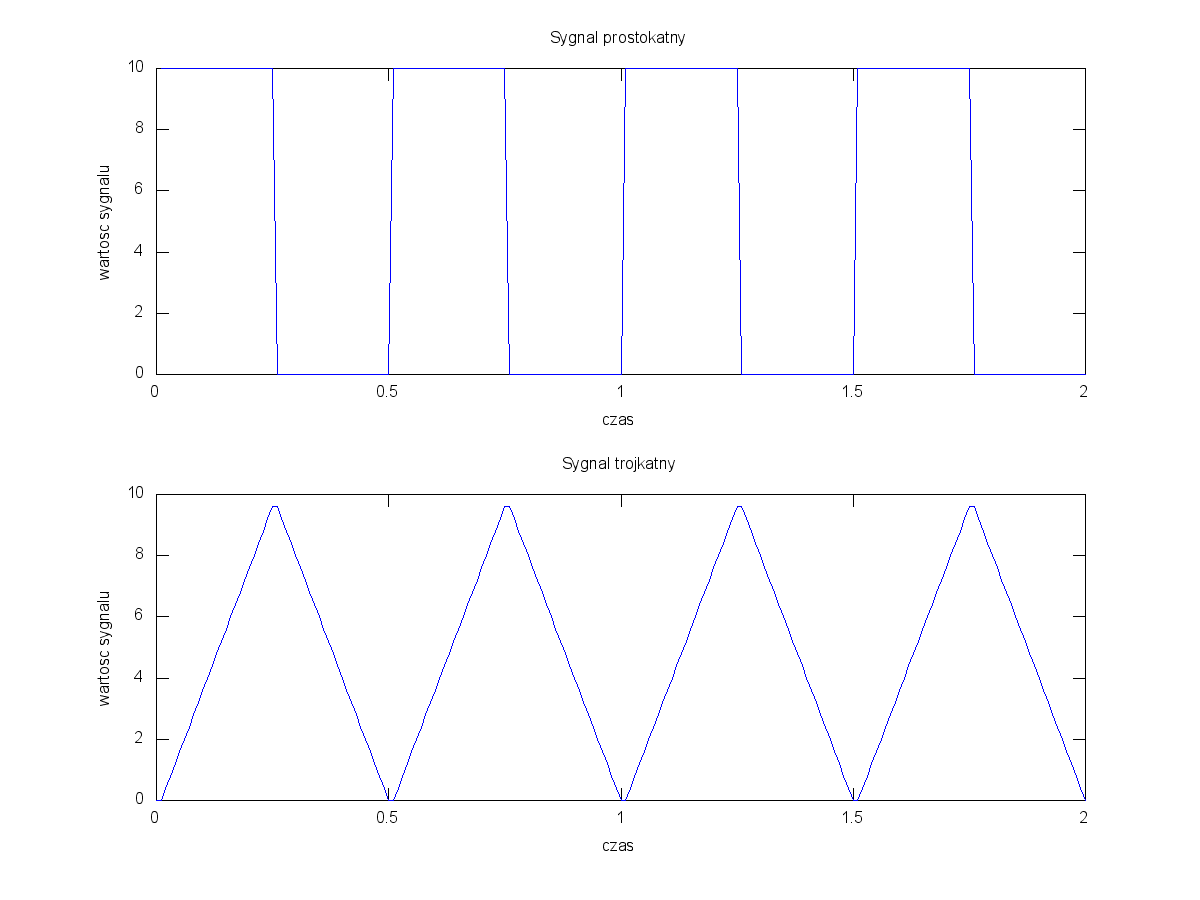
\includegraphics[scale=.5]{out/Figure1.png}
  %       \caption{\label{wykres1}Badane sygnały.}
  %     \end{center}
  %   \end{figure}
  % \end{landscape}
  
% Wykresy (end)
\end{document}